\Chapter{Fesztivál alkalmazások}

Az elkészülő alkalmazás specifikációja előtt érdemes áttekinteni, hogy pontosan milyen szolgáltatások kapcsolódnak egy fesztiválhoz. Ez segít majd behatárolni az alkalmazás szükséges funkciót. Fontos továbbá ennek kapcsán megvizsgálni, hogy milyen hasonló alkalmazások érhetők már el, illetve azok milyen feladatokat és milyen formában látnak el.

\Section{Fesztiválokhoz kapcsolódó szolgáltatások}

Először nézzük meg, hogy pontosan hogyan definiálhatnánk, hogy mi tekintünk fesztiválnak.

„Fesztiválnak nevezhető minden olyan – egy vagy több
téma köré szerveződő, rendszeresen megrendezésre
kerülő, egy vagy több helyszínen történő, meghirdetett
programmal rendelkező kulturális, művészeti, gasztronómiai,
sport vagy egyéb – eseménysorozat, amelynek
célja, hogy közönsége részére kiemelten színvonalas,
értékközvetítő, minőségi, ismereteket is bővítő és egyben
szórakoztató, szabadidős közösségi élményt nyújtson.”
(Magyar Fesztivál Szövetség \cite{21})

A hazai turizmus bevételeinek jelentős részét a program azon belül a fesztiválturizmus adja.

A fenti kijelentésemet bizonyítja két interneten talált cikk is, melyek viszonylag frissek voltak a témában. Az egyikből kiderül, hogy Magyarországon több mint 9000 fesztivált rendeznek egy év alatt és ezeknek 40 százaléka vonz tízezer főnél több látogatót. Jellemzően magyarok látogatják ezeket. A fesztiválok jelentősen megnyújtják a turisztikai főszezont és csökkentik a turizmusforgalom Balaton-Budapest központúságát. A magyar lakosság harmada lelkesedik a fesztiválokért. Jelentős részük a fiataloknak szól, így a 15-30 éves kor között a számarányuk a duplája is lehet.(turizmus.com Dübörög a fesztiválturizmus cikke alapján \cite{16}). 
A külföldi látogatók alapján a Sziget fesztivál a Balaton Sound és a VOLT fesztivál kiemelkedőek, Sorrendben 85-45-10\%-os külföldiek részaránya. Csak a Szigetnek köszönhetően 300 ezer vendég éjszakát töltöttek az országban a külföldi turisták. A fesztiválok az országba irányuló turizmus 10-12\%-át adják és évi 100 milliárdos bevételt generálnak a gazdaság számára \cite{15}.

A dolgozatomban a klasszikus értelembe vett zenei vagy zenei vonatkozású fesztiválokra fókuszálok.
A fesztiválokhoz nagyon változatos és sokrétű funkció csoportok tartoznak, melyeket több szempont alapján kategorizálhatunk. Az elkészülő szoftver funkcióinak behatárolásához, a követelményspecifikáció elkészítéséhez vegyük ezeket sorra.

\SubSection{Közvetlenül kapcsolódó funkciók}

A fesztiválozáshoz, mint szolgáltatáshoz közvetlenül kapcsolódó funkciók az alábbiak.
\begin{itemize}
\item Koncertek, a legnagyobb vonzereje a fesztiválnak. A koncert szolgáltatást a fellépők nyújtják a résztvevők számára, gyakran több színpadon párhuzamosan. Ezeket kellő időben és helyen kell megismertetni a közönséggel. Ide értve nem csak a zenei produkciókat, de egyéb performance-t, és előadásokat, prevenciókat.
\item Élelmiszer és ital árusítás. Alapvető szükségletet elégít ki, mivel a zenei fesztiválok jelentős része 3-10 napos periódusban gondolkodik, így jelentős összeget költenek erre a kategóriára. Gyakran többet mint magára a belépőre, utazásra, szállásra.
\item Egyéb sport, kulturális, szellemi programok, vetélkedők. Technológiai bemutatók kipróbálási lehetőséggel.
\item VIP szolgáltatások, közönségtalálkozók.
\item Szállási lehetőségek a fesztivál területen.
\end{itemize}

\SubSection{Közvetve kapcsolódó funkciók}

Közvetve kapcsolódó funkciók: Amelyeket nem érzékel, amikért nem fizetne önmagában, illetve nem kell tudnia a fesztiválozónak, de kényelmetlenül érezné magát, ha nem valósulnának meg. Ilyenek például az alábbiak.
\begin{itemize}
\item Takarítás, WC használat, zuhanyzási és alvási lehetőség.
\item A színpadok, dekorációk, kerítések építése, karbantartása, lebontása.
\item A fellépők oda és haza juttatása zökkenőmentesen.
\item Készletgazdálkodás, promóciók, kérdőívek.
\item Média megjelenés.
\item Elektronikus, internetes hálózat, közvilágítás.
\item Biztonság, az időjárás viszontagságai ellen védelem, értékmegőrzés.
\item Rekreáció, egészségmegőrzés.
\item Fodrász, kozmetikus a feltűnő és kreatív megjelenés érdekében.
\item Véradásért cserében valamilyen ellenszolgáltatás.
\end{itemize}

\SubSection{Az alkalmazás szempontjából kiemelt funkciók}

Melyek azok a szolgáltatások, amelyek érdekelni fogják a felhasználót, szeretne előretudni róla, és ezeket egy információs rendszerben meg lehet jeleníteni.
\begin{itemize}
\item Fellépők listája, mint már említettem ez az egyik legfőbb vonzerő.
\item Az extrém nem mindenhol kipróbálható sportolási, technológiai lehetőség.
\item Hasznos lehet a környékbeli étkezők elérhetősége, akár étlapja árakkal. Tudjuk, hogy a fesztiválok a magas áraikról és főleg a gyors étkezdéikről híresek. Érdemes lehet az olcsóbb, vagy a gasztronómia szerelmeseinek a környező elit éttermekről előre információt nyújtani.
\item Dohányboltok, illetve dohányzás. Magyarországon jelenleg a jogszabályi környezet befolyásolja a dohányáruk vásárlási helyét, erről nyújthat információt egy alkalmazás, és arról is, hogy lehetséges-e dohányozni a fesztiválterületen vagy sem.
\item Szállás, vannak olyan fesztiválok, amelyek sátorhelyet és/vagy faházat biztosítanak a közönségük számára. Emellett megjeleníthetőek a kollégiumok, apartmanok, szállodák.
\item Kutyabarátság, kutya bevihető-e a rendezvényre.
\item Gyerekbarátság, gyermekek bevihetőek-e, esetleg vannak-e számukra külön programok.
\item Jegyek, kell-e fizetnünk a fesztiválra belépésért vagy ingyenesen látogatható. Ha igen, akkor milyen jegytípusok érhetőek el.
\item Strandolási lehetőség. A zenei fesztiválok jelentős része nyáron van és vízközelben, hogy a közönségnek legyen lehetősége védekezni a meleg ellen.
\end{itemize}

\SubSection{Konkurens alkalmazások}

Az interneten fellelhető már egypár elterjed Fesztivál/Esemény kereső alkalmazás, vannak hiányosságaik és tartalmaznak frappáns ötleteket is. A következő szakaszok ezeket tekintik át.

\SubSection{Fesztiválkalauz.hu}

\texttt{http://www.fesztivalkalauz.hu}. Az első dolog amivel a felhasználó találkozik az a felhasználói felület, amelynek körülbelül a felét használta ki a fejlesztő. Jelenleg egy 14"-os kijelzőn nézve ez zavaróan kicsi. Feltehetőleg ez azért is van így, mert nagyjából 10 éves fejlesztés, és akkor még nem volt ekkora kijelző választék - sem méret, sem eszköz tekintetében - amelyeken weboldalakat jelenítettünk meg, így elég volt egy statikus méretre és betűtípusra beállítani a weboldalt. Jelenleg divatosak a reszponzív weboldalak, amelyek igyekeznek kiküszöbölni ezt a problémát.

A reszponzív kialakítás manapság alapelvárásnak tekinthető \cite{1}. Ez főként azért lényeges, mert az eddigi, klasszikus értelemben vett webböngészős megjelenítés mellett különböző eszközök, különböző képernyőméretekkel és arányokkal teszik elérhetővé a tartalmakat. Törekedni kell arra, hogy átméretezést követően is áttekinthető és kezelhető maradjon a felhasználói felület.

A viszonylag fejlett fesztiválkereső nekem tetszik, sok mindenre rálehet keresni, könnyen és átláthatóan. Lehet település, kerület, illetve megye szerint is keresni. Típus és dátum szerinti keresés is támogatott. Sőt módunkban áll a következőhavi eseményeket is lekérdezni egy kattintással, erről ha szeretnénk, hírlevelet is kérhetünk. A szabad szavas kereső, annyira azért mégsem szabad, mert csak a címben keres a leírásban sajnos nem.

\SubSection{Utazzithon.hu}

\texttt{https://www.utazzitthon.hu/program}. Az oldal mint a szlogenje is mondja: "Belföldi szállás, program és látnivaló 1 helyen", szállásokat és programokat közvetít az érdeklődőknek. A felület már reszponzív tervezés eredménye, ennek köszönhetően átlátható és könnyen használható akár mobileszközről is. A keresés nagyon világos, kereshetünk régió, tájegység, város szerint és program, látnivaló típusok alapján. Az adatbázisuk programok tekintetében elég gazdag, amikor megtekintettem közel 8000 programot ajánlottak. Itt jegyet is vásárolhatunk az egyes programokra.

\SubSection{Fesztival.eu}

\texttt{http://www.fesztival.eu}. A weboldal régi dizájnnal készült. A keresője nagyjából hasonló funkciókat tükrözött, mint az eddigiekben megjelenő keresési lehetőségek. Sajnos az adatbázisában csak egy fesztivál volt megtalálható, amikor ott jártam, így tesztelni nem volt módom.

\SubSection{Fesztiválnaptár.hu}

\texttt{http://www.fesztivalnaptar.hu}. Az iranymagyarorszag.hu által működtetett weboldal. Feltehetően az utazzitthon.hu-hoz hasonlóan a szállások közvetítése a főprofilja, és ezek mellé jönnek be a fesztiválok, koncertek mint kiegészítőszolgáltatások. Szabad szavas kereséssel és kronológiai sorrend szerinti érhetőek el a programok. A szabad szavas kereső viszont keres a leírásban is, ami sokat könnyít a felhasználó számára. A felület nem reszponzív és régebbi stílusú. Nem nagy meglepetés, hogy 100-nál kevesebb esemény programját találjuk meg. Itt jelenik meg egyedül a nemzetköziesítés, a magyaron kívül angolul és németül is elérhetőek a programok, habár a programokhoz tartozó leírások csak magyarul érhetőek el.

\SubSection{Programturizmus.hu}

\texttt{https://www.programturizmus.hu}. Az utolsó, keresést támogató rendszerhez érkeztünk amit találtam, és szerintem a legletisztultabb felülettel és szolgáltatásokkal. Természetesen modern weboldal lévén, platformtól és kijelző mérettől függetlenül szépen megjelenik bármilyen eszközön. Az oldal nem csak fesztiválokra, hanem szinte minden olyan lehetőséget hivatott bemutatni, ami kimozdítja a fotelból a felületen böngésző felhasználót, ez a hozzáállás a szlogenben is tükröződik - ,,Ne maradj otthon''. Találunk itt a vásárok, látnivalók, és gasztronómián belül, Kolbásztöltő versenytől, a Kutyakiállításon át a Régiségvásárig mindent. Persze megjelennek a már klasszikusnak mondható szállások is. A keresés a már az előzőekben megszokott lehetőségek szerint lehetséges. Viszont az "Események" mellett megjelenik három új lehetőség is, az egyik az "Ajánlat" menü, a másik az "Érdekesség", ezek valami alapján kitüntetett események, viszont az utolsó talán a legérdekesebb. Ez pedig a koordináták alapján megmutatja, hogy hol is lesznek helyileg az események egy google térképen. A jegyet itt is vásárolhatunk. Ha egy fesztivált részletesebben megnézünk, meglepőmódon a jegyen, a címen és szálláson kívül még a környékbeli étkezési lehetőségeket is tanácsolja számunkra a weboldal.

\SubSection{Élményem.hu}

\texttt{http://elmenyem.hu}. Az oldal nem rendelkezik fesztiválkereső résszel. Ez inkább egy blog, de rengeteg aktualitással, hírekkel szolgál a jövőben megrendezendő eseményekkel kapcsolatban. 

\Section{Weboldalak összegzése}

A fenti oldalakról a paramétereik alapján egy táblázatot készítettem (\ref{fig:apps}. ábra).

\begin{figure}
\centering
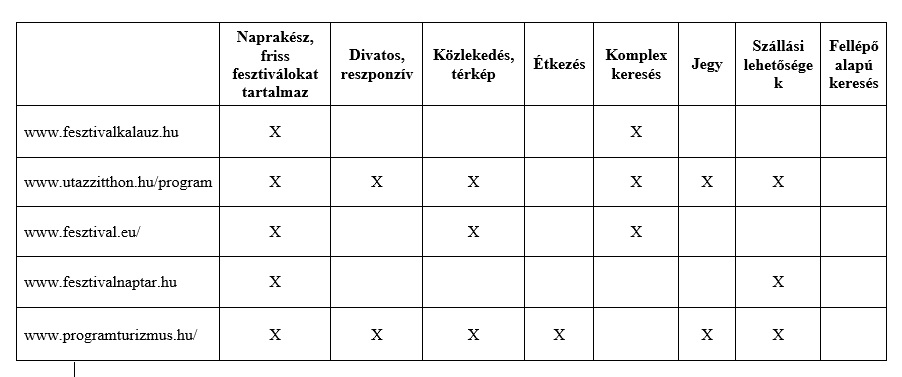
\includegraphics[scale=0.64]{kepek/alkalmazasok.jpg}
\caption{Alkalmazások funkciói táblázatos formában}
\label{fig:apps}
\end{figure}

Ezek szerint mindegyik naprakész információkat tartalmaz, habár a fesztivál.eu-n megjelennek olyan fesztiválok is amelyek már régen véget értek.

Csak két weboldal dizájnja a kornak megfelelő, amelyek a utazzitthon.hu és a programturizmus.hu.

A Fesztiválokat térképen való megjelenítésére már weboldal is gondolt, ahogy ezt a táblázatról leolvashatjuk.

Étkezéssel kapcsolatos információkat csak a programturizmus oldalán találhatunk.

Összetettebb kereséseket az első három weboldalon készíthetünk.

Jegyvásárlásra vagy a jegyvásárlási lehetőségekhez való eljutáshoz ugyanaz a két oldal biztosít lehetőséget, amely reszponzív webdizájnt is alkalmaz.

Szállási lehetőségeket a fesztiválkalauz és a fesztivál.eu-n kívül mindegyik weboldalon találunk.

Fellépő alapú keresést sajnos egyik oldal sem szolgáltat számunkra.

\Section{További lehetséges szolgáltatások}

Az itt felsorolt weboldalak természetesen a jövőben változásokon eshetnek át. Ezek a szakdolgozat írás közbeni állapotokat tükröznek.

Extra lehetőségek, amelyekkel nem éltek az itt feltüntetett weboldalak:
\begin{itemize}
\item SZÉP-kártya, és egyéb fizetési lehetőségek feltüntetése.

\item Gyerek illetve kutyabarát-e a rendezvény. Könnyen megvalósítható, mégis látványos lehetőségeket rejt magában, hiszen egy cumi, vagy egy mancs elhelyezése az esemény mellett vagy alatt, adatbázis szinten pedig csak egy boolean változó bevezetése.

\item Dohányzásra, alkoholfogyasztásra, korhatárra is lehetne bevezetni hasonló kis ikonokat, ezeket is egyszerű paraméterként fel lehetne szerelni.

\item Értékmegőrzésre, telefon töltésre van-e lehetőség. 

\item Ingyenes-e a rendezvény: Ez is könnyen felkeltheti az érdeklődők figyelmét. Itt is alkalmazható lenne a már jól bevált ikonos megoldás.

\item A nemzetköziesítés is szempont lehet, habár ezek az oldalak elsősorban hazai piacra készültek, amelyek fesztiválok nemzetközi vendégeket várnak, azoknak a marketingprogramja is külföldre pozíciónál, és saját weboldallal is rendelkeznek. Ideértve az árak több valutában való megjelenítését is a leírások szövege mellett.

\item Közlekedés: Érdemes lehet feltüntetni, magát a fesztivál koordinátáit, mint ezt a programturizmus.hu weboldalon láthattuk, emellett érdemes lehet parkolási lehetőségekről térképen előre informálni az odaérkezőket, egy nagyobb eseményre akár több ezer személyautóval is érkezhetnek. A buszpályaudvarról és vasútállomásról a célhoz eljutást segítő helyi járatok menetrendjét is lehetne mellékelni. Az eseménnyel szerződött taxivállalatok telefonszámait felsorolni. A gyalogos eljutást térkép segítségével megmutatni.

\item Szállás: Mint láthattuk, majdnem mindegyik weboldal ajánlott szállást hotelekben, de a fesztiválok klasszikus közönsége, az nem szállodákban alszik. Általában sátorban, faházakban, kollégiumokban, vagy épp ahol eléri az álom. Érdemes lenne jelezni a felhasználó felé, hogy lehet-e sátrazni, és ha igen, van-e ennek extra költsége. A kollégiumokat, faházakat is lehetne ilyen módon jelezni.

\item Időjárás: Ez sajnos nem jósolható hónapokkal előre, de pár héttel a fesztivál kezdete előtt ez is felkerülhetne. Hisz mint tudjuk, ezen események javarészt fedetlen vagy részben fedett helyeken zajlanak.

\item Visszacsatolás: A legtöbb ilyen eseményt többször megrendezik, vannak olyanok amik már 20-30 éves hagyományra tekintenek vissza. Így az értékelések, mind a szervezők, mind a szolgáltatást igénybe vevők számára hasznos információt nyújtanak.

\item Étkezés: Amire csak a \textit{programturizmus.hu} gondolt, és alapvetően egy jó kis kiegészítő szolgáltatás, hisz fiziológiai szükségletet elégít ki.

\end{itemize}

\Section{Differencia az eddig létező és a saját alkalmazásom között}

Az eddigiek alapján meg kell határozni, hogy miket szeretnénk, ha megvalósítana az alkalmazásunk, miben lesz más vagy jobb mint a többi a piacon fellelhető alkalmazás. Én igyekszem két új aspektust bevezetni, amelyeket ott nem, vagy nem egészen így alkalmaztak. Az egyik a fellépő alapú szemlélet. Szeretném, ha nemcsak a fesztiválról tudnánk meg többet, hanem az ott fellépő zenekarokról is érhetnénk el információkat. Ha nem ismerem őket, akkor rákattintva megtudhatok róluk pár információt, illetve az oldalra felvitt fesztiválok alapján a turné állomásokat. A másik aspektus a kulcsszavak bevezetése mint fesztivál, mint fellépő oldalon. Hasonlóval találkozhattunk egy-két általam is bemutatott oldalon. Amilyen paraméterek számításba jöhetnek: zenei stílusok, fesztivál stílusok, sátrazási lehetőség, kutyabarát. A divatos nevén a hashtag-ek. Adatbázis és program szinten stílusnak nevezem el, de talán ez egy kicsit tágabb fogalom. A következő fejezetben ezeket részletezzük is.
